\section{Medical Rationale (Sophie)}
\label{sec:medicalneed-sophie}
Medical rational for the app can essentially be split down into two areas: prevalence i.e. how many people suffer; and prognosis, likely course of the condition. There is additional supporting evidence for a preliminary diagnostic app for obstructive sleep apnoea, some of which is discussed below

The British Lung Foundation has prioritised OSA and created an OSA Charter calling on the UK governments to make OSA a national priority as well as encouraging investment in research. They held a three year campaign to raise awareness which ended in 2014. The campaign had two aims: to increase awareness by both the general public and health care professionals and to improve diagnosis. Part of the plan to improve diagnosis was to develop a national standard for diagnosis that would include a “one-stop shop for treatment set-up [to] shorten the total patient pathway, especially from diagnosis to treatment, [to] reduce concerns about driving”. A conference on OSA was held in February 2014 where doctors expressed a desire to change the current system, due to increased need for doctor referral of patients to sleep centres ~\cite{britishlungfoundation}.

PhysioNet and Computers in Cardiology, with funding from Margret and H.A. Rey Laboratory for Nonlinear Dynamics in Medicine, set up a competition with two prizes of \$500 for whoever could classify ECG data, obtained minimally intrusively and inexpensively, into that from OSA sufferers and normal subjects, with the intension of using it as a screening tool ~\cite{physionet}.

The Agency for Healthcare Research and Quality felt that the diagnosis of sleep apnoea was a sufficiently important public health issue that they commissioned a study on future research needs which includes a reference to the need for portable monitors, including limited-channel, low-cost portable devices ~\cite{balk2012future}.

\subsection{Prevalence}
Prevalence of OSA is hard to know due to the fact a high levels of cases go undiagnosed (up to 90\% of cases~\cite{finkel2009prevalence}), however estimates range from 1 to 28\% of the adult population depending on severity and location ~\cite{young2002epidemiology}.

There may be an ethnicity element in prevalence, however few studies have been undertaken other than in western countries and therefore prevalence elsewhere is essentially unknown. For some areas it is known, this means studies on causes can be undertaken. For example prevalence in Western Nations and Hong Kong is very similar but prevalence of risk factors is very different: there are high levels of obesity in the west but not in those studied from Hong Kong, so hypotheses have been produced on other risk factors including facial features being more prevalent in Hong Kong and some clinical observations support these hypotheses ~\cite{ip2001community}.

Gender has been shown to have an effect with estimates of 2 to 3 times greater risk for men compared to women; the reasons behind this are unclear ~\cite{strohl1996recognition}. Hormones have been considered but administration of the female hormones oestrogen and progesterone to men does not appear to have an effect ~\cite{shaver2000review}. Men show greater prevalence to many chronic diseases so this may be part of a greater trend and differences elsewhere have been shown to be linked to physical features, occupation, environment, attitude to health, and risky behaviour. There are gender differences in upper airway shape, muscle activity, facial shape, and deposition of fat in the airway, however the few studies that have looked at this have yet to find a conclusive link. Occupation, attitude to health and risky behaviour have not been studied in the context of gender disparity in OSA sufferers ~\cite{waldron1985we}.

There are hypotheses proposing higher prevalence of OSA in pregnant mothers but few data sets to support this. Proposed mechanisms to cause this include excess weight gain and the effect of sleep deprivation on pharyngeal dilator muscle activity ~\cite{franklin2000snoring}.

Although a positive correlation between OSA prevalence and age appears to exist for mid life, the same is not true for younger or older patients. OSA in children has similar consequence to that in adults and some of the pathophysiology (physical manifestation of the disease) is the same, however the etiology (causes) and associated morbidity (rate of incidence of the disease) can be very different, which means that it is generally studied independently from the adult form ~\cite{ancoli1991sleep}.

In old age prevalence of OSA increases, however this does not necessarily mean that physiological changes associated with old age are causing OSA. If this was the case one would expect the prevalence rate to increase at the same rate as through middle age or at a higher rate. Figure \ref{fig:prevalence} shows the Sleep Heart Health Study on prevalence with age which starts to flatten in the 60s which suggests age related prevalence tails off at this point ~\cite{young1996sleep}.

\begin{figure}[h]
\centering 
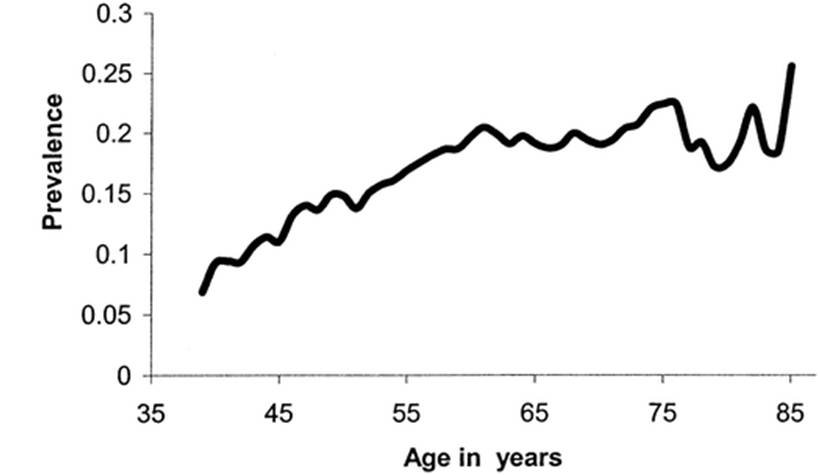
\includegraphics[width=0.5\textwidth]{drawings/prevalenceage}
\caption{Prevalence of OSA by age in the Sleep Heart Health Study ~\cite{young2002predictors}.}
\label{fig:prevalence}
\end{figure}

It is possible that older age OSA is actually distinct from that of middle age. Several studies support this theory, as many of the key symptoms of middle age OSA are not present in the old age version, including daytime sleepiness, obesity, decrease in cognitive function and hypertension. Snoring is also significantly less reported, however this could be caused by increase in bed partner hearing loss and death ~\cite{enright1996prevalence,young1996sleep}.

\subsection{Prognosis}
The prognosis for sufferers of OSA can be quite severe, with many suffering with secondary conditions such as hypertension. Cognitive function is also impaired and most suffer from daytime sleepiness which effects ability to drive and hold down a job.

There is an association between OSA and secondary hypertension (high blood pressure) independent of excess weight and other factors. This link is seen even in mild OSA, and given the prevalence of OSA could be having an impact on a significant proportion of those suffering with hypertension. However attempts to treat OSA in order to reduce hypertension have so far yielded unclear results ~\cite{pankow2000sleep}.

Hypertension is linked to cardiovascular and cerebrovascular disease, and given the link between OSA and hypertension, OSA will moderately contribute to the morbidity and mortality of these. There may also be direct links between OSA and cardiovascular disease however this has been less well studied. Whether treatment of OSA can improve cardiovascular disease has yet to be assessed ~\cite{he1988mortality}.

Daytime sleepiness is a primary feature of OSA and many studies have shown that treatment of OSA does reduce daytime sleepiness ~\cite{ballester1999evidence}. Studies have found a significant association between snoring and daytime sleepiness ~\cite{engleman1999randomized,stradling1991self}.

The effects of OSA on cognitive function is not fully understood. There are some population based studies which find weaker correlations than clinic based studies. This is probably due to the biased population who attend sleep laboratories. In one study OSA was significantly but weakly related to reduced psychomotor efficiency (a measure of coordination of fine motor control with sustained attention). This link was not explained by daytime sleepiness ~\cite{kim1997sleep}. In another study of self reported snorers a weak but significant association was found between OSA and neuropsychological function ~\cite{adams2001relation}. One suggested mechanism for reduction in cognitive function is due to oxygen starvation in the brain during apnoeas. This can change neurons especially in the hippocampus and right frontal cortex and so far has not seen improvement with treatment of OSA ~\cite{gale2004effects}.

There is no specific quality of life measure for OSA although one is being developed. However the SF-36, a general health-related quality of life measure, a short form of the Medical Outcomes Study, is in use. A couple of studies have found a linear association between severity of OSA and decrements on the SF-36 scales, showing undiagnosed OSA has a similar affect on quality of life to other chronic disorders of similar severity. However another study showed a threshold effect as severity of OSA increased, however a small sample size limits usability ~\cite{finn1998sleep,baldwin2001association}.

Patients with OSA have a higher vehicle crash rate than the general population. This has been shown by crash records, self-reports and performance on driving simulators. This is a significant issue because it puts the lives of everyone not just the sufferers at risk. Studies undertaken in clinic will over estimate rate of crashes due to selection bias, however there are population studies looking at those with undiagnosed OSA which also show a strong correlation, especially among men. Self-reported sleepiness was not able to explain the crash rate. This is concerning because it means those at risk are not able to recognise it within themselves and are therefore unable to take precautions to reduce risk ~\cite{findley1988automobile,findley1989driving}.
